\documentclass[runningheads,a4paper]{llncs}

\usepackage{amssymb}
\setcounter{tocdepth}{3}
\usepackage{graphicx}
\graphicspath{{./figs/}}

\usepackage{amsmath} 
\usepackage{bm}
\usepackage{amsbsy} 
\usepackage{amssymb}
\usepackage{cite}

\usepackage{color, colortbl}
\definecolor{col1}{gray}{0.8}
\definecolor{col2}{gray}{0.9}
\definecolor{col3}{gray}{0.95}


\newcommand{\keywords}[1]{\par\addvspace\baselineskip
\noindent\keywordname\enspace\ignorespaces#1}

\newcommand{\grad}{\mathop{\rm grad}\nolimits}
\newcommand{\const}{\mathop{\rm const}\nolimits}
\renewcommand{\div}{\mathop{\rm div}\nolimits}
\newcommand{\half}{\frac{1}{2}}

\title{Solution of the 3D Neutron Diffusion Benchmark by FEM}

\author{A.V. Avvakumov$^{1}$, P.N. Vabishchevich$^{2}$, A.O. Vasilev$^{3,a)}$ and V.F. Strizhov$^{2}$}

\institute{$^1$National Research Center \emph{Kurchatov Institute}, Moscow, Russia \\
$^2$Nuclear Safety Institute of RAS,  Moscow, Russia \\
$^3$North-Eastern Federal University, Yakutsk, Russia\\
$^{a)}$Corresponding author: \url{haska87@gmail.com}}

\titlerunning{Solution of the 3D Neutron Diffusion Benchmark by FEM}
\begin{document}

\maketitle

\begin{abstract}
The objective is to analyze the neutron diffusion benchmark developed by the Atomic Energy Research community for verification of best-estimate neutronics codes. 
The 3D benchmark of Schulz models a VVER-1000 core in steady state. 
The assemblies are homogeneous, represented by given diffusion theory parameters. 
There are seven material compositions including four enrichments, burnable absorber, control rods and a reflector. 
The finite element method on tetrahedron computational grids is used to solve the three-dimensional neutron problem. 
The software has been developed using the engineering and scientific library FEniCS. 
The matrix spectral problem is solved using a scalable and flexible toolkit SLEPc. 
The solution accuracy of the benchmark is analyzed by condensing the computational grid and varying the degree of the finite elements.
\end{abstract}

%\keywords{Neutron diffusion equation, multi-group approximation, space-time kinetic, spectral problem.}


\section{Introduction}
The physical processes in a nuclear reactor \cite{duderstadt1976nuclear}
depend on the distribution of the neutron flux, whose mathematical description is based on the neutron-transport equation \cite{hetrick1971dynamics,stacey2007}. 
The equation, describing the process is of integro-differential form and the required distribution of neutrons flux depends on time, energy, spatial and angular variables. As a rule, simplified forms of the neutron transport equation are used for practical computations of nuclear reactors. The system of equations obtained by the multigroup diffusion approach is often used for reactor analysis \cite{marchuk1986numerical,lewis1993computational} and is applied in most engineering calculation codes.
%sutton1996diffusion,cho2005fundamentals

The processes in a nuclear reactor are essentially non-stationary. The stationary state of neutron flux, which is related to the critical state of the reactor, is characterised by local balance between the neutron generation and absorption. This boundary state is usually described by the solution of a spectral problem (Lambda Modes problem, $\lambda$-eigenvalue problem) provided that the fundamental eigenvalue (the maximal eigenvalue) that is called k-effective of the reactor core, is equal to unity. In this case, the stationary neutron flux is a corresponding eigenfunction. Computations of k-effective of the reactor using the Lambda Modes problem are obligatory for reactor design calculations.

To verify neutron diffusion codes several benchmark problems have been developed. This work is focused on the solution of the 3D benchmark problem of a VVER-1000 core in steady state. Convergence of the benchmark solution is under investigation.

\section{Problem description}

Let's consider modelling neutron flux in a multi-group diffusion approximation. Neutron flux dynamics is considered within a bounded 2D or 3D domain  $\Omega$ ($\bm x = \{x_1, ..., x_d\} \in \Omega, \ d = 2,3$) with a convex boundary $\partial \Omega$. The neutron transport is described by the following set of equations without taking into account delayed neutron sources:
 \begin{equation}\label{1}
\begin{split}
 \frac{1}{v_g} \frac{\partial \phi_g}{\partial t} - & \nabla \cdot D_g \nabla \phi_g + \Sigma_{rg} \phi_g 
 - \sum_{g\neq g'=1}^{G} \Sigma_{s,g'\rightarrow g} \phi_{g'} \\
 =  & \ ( (1-\beta) \chi_g + \beta \widetilde{\chi}_g) \sum_{g'=1}^{G} \nu \Sigma_{fg'} \phi_{g'} , \quad 
 g = 1,2, ..., G .
\end{split}
\end{equation} 
Here $\phi_g(\bm x,t)$ is the neutron flux of group $g$ at point $\bm x$ and time $t$,
$G$ is the number of groups,
$v_g$ is the effective velocity of neutrons in the group $g$,
$D_g(\bm x)$ is the diffusion coefficient, $\Sigma_{rg}(\bm x,t)$ is the removal cross-section,
$\Sigma_{s,g'\rightarrow g}(\bm x,t)$ is the scattering cross-section from group $g'$ to group $g$,
$\beta$ is the effective fraction of delayed neutrons, $\chi_g$, $\widetilde{\chi}_g$  is the spectra of instantaneous and delayed neutrons, 
$\nu\Sigma_{fg}(\bm x,t)$ is the generation cross-section of group $g$.
The conditions so-called albedo-type are set at the boundary $\partial \Omega$:
\begin{equation}\label{2}
 D_g\frac{\partial \phi_g}{\partial n} + \gamma_g \phi_g = 0, \quad 
 \quad g = 1,2, ..., G ,
\end{equation}
where $n$ is the outer normal to the boundary $\partial \Omega$.
Let's consider problem (\ref{1}) with boundary conditions (\ref{2}) and initial conditions
\begin{equation}\label{3}
 \phi_g(\bm x,0) = \phi_g^0(\bm x), 
  \quad  g = 1,2, ..., G .
\end{equation} 

We write the boundary problem (\ref{1}), (\ref{2}), (\ref{3}) in operator notation. 
We define the vector $\bm \phi = \{\phi_1, \phi_2, ..., \phi_G\}$ and the matrices
\[
 V = (v_{g g'}),
 \quad v_{g g'} = \delta_{g g'} v_g^{-1},
\] 
\[
 D = (d_{g g'}),
 \quad d_{g g'} = - \delta_{g g'} \nabla \cdot D_g \nabla,
\] 
\[
 S = (s_{g g'}),
 \quad  s_{g g'} =  \delta_{g g'} \Sigma_{rg} - \Sigma_{s,g'\rightarrow g} ,
\] 
\[
 R = (r_{g g'}),
 \quad  r_{g g'} = ( (1-\beta) \chi_g + \beta \widetilde{\chi}_g) \nu \Sigma_{fg'} ,
\]
\[
g, g' = 1,2, ..., G,
\] 
where
\[
 \delta_{g g'} = \left \{ 
 \begin{matrix}
 1, & g = g', \\
 0, & g \neq  g',
 \end{matrix}
 \right . 
\] 
is the Kronecker delta. Consider the set of vectors $\bm \phi$,  whose components satisfy the boundary conditions
(\ref{3}). Using the above introduced definitions, the system of equations (\ref{1}) takes in the form of the first-order evolutionary equation
\begin{equation}\label{4}
 V \frac{d \bm \phi}{d t} + (D+S) \bm \phi = R \bm \phi .
\end{equation}  
We solve the Cauchy problem for (\ref{4}), when
\begin{equation}\label{5}
 \bm \phi(0) = \bm \phi^0,
\end{equation} 
where $\bm \phi^0 = \{ \phi_1^0,  \phi_2^0, ...,  \phi_G^0 \}$.

To characterize the dynamic processes in a nuclear reactor, which are described by the Cauchy problem (\ref{4}), (\ref{5}), solutions of some spectral problems (see \cite{publicAnnnals2017}). Let's consider the solution of the spectral problem, called Lambda Modes problem:
\begin{equation}\label{6}
 (D+S) \bm \varphi  = \lambda^{(k)} R \bm \varphi .
\end{equation} 
Problem (\ref{6}) is known as the Lambda modes problem for a given configuration of the reactor core.
The minimal eigenvalue is used for characterisation of neutron flux, thus 
\[
 k = \frac{1}{\lambda^{(k)}_1}  
\] 
is the effective multiplication factor (see \cite{stacey2007}).

\section{AER Benchmark}
The 3D benchmark, Schulz \cite{schulz1996}, models a VVER-1000 core in a steady state. The assemblies are homogeneous, represented by given two-group diffusion theory (see more \cite{duderstadt1976nuclear}, \cite{stacey2007}) parameters. There are seven material compositions including four enrichments, burnable absorber, control rods and reflector. The core height is 355 cm, covered with axial and radial reflectors. The nodes are large, with assembly lattice pitch of 24.1 cm. Figure \ref{fig:1} shows the radial and axial model geometry.  Diffusion neutronics constants in the common notations
are given in Table \ref{t-1}. 

%\begin{figure}[htp]
%  \begin{center}
%    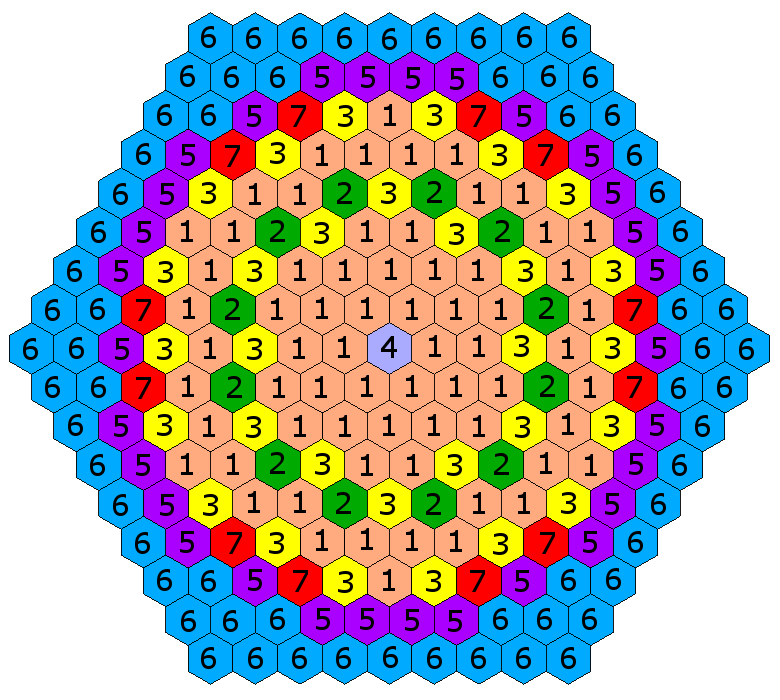
\includegraphics[width=0.45\linewidth] {1.png}
%	\caption{Radial geometry model}
%	\label{fig:1}
%  \end{center}
%\end{figure} 
%
%\begin{figure}[htp]
%  \begin{center}
%    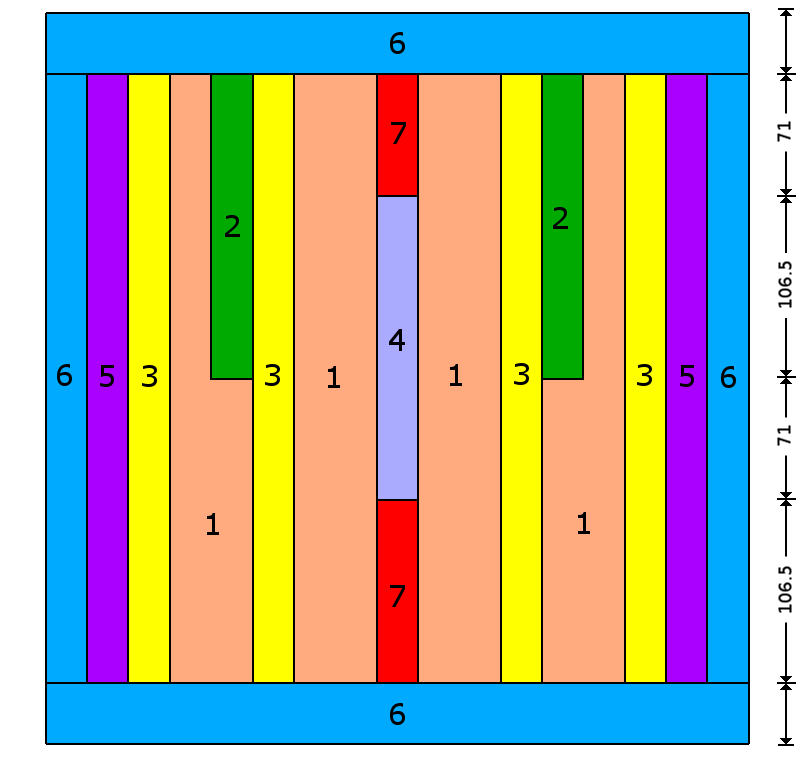
\includegraphics[width=0.45\linewidth] {2.png}
%	\caption{Axial geometry model}
%	\label{fig:2}
%  \end{center}
%\end{figure}

\begin{figure}[h]
\begin{center}
\begin{minipage}{0.48\linewidth}
\center{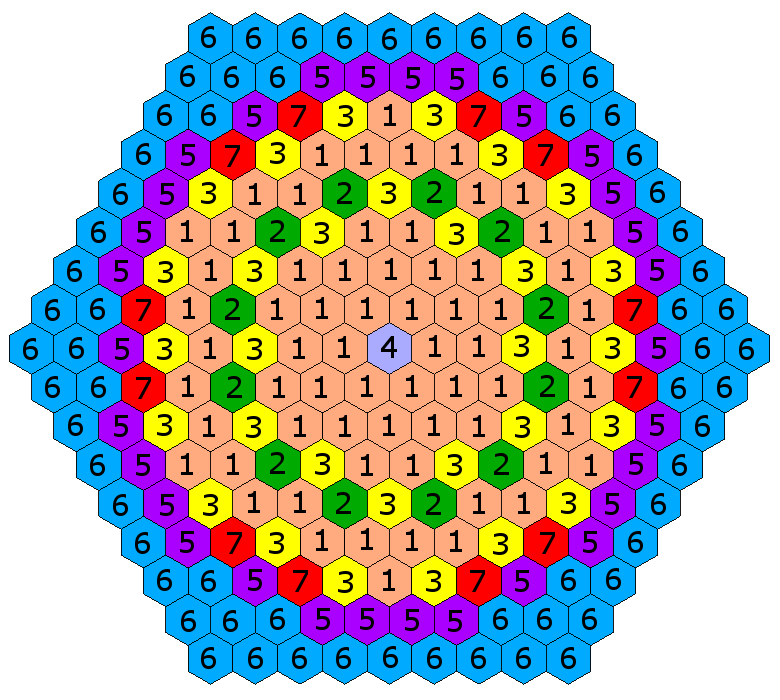
\includegraphics[width=1\linewidth] {1.png}}\\
\end{minipage}
\hfill
\begin{minipage}{0.48\linewidth}
\center{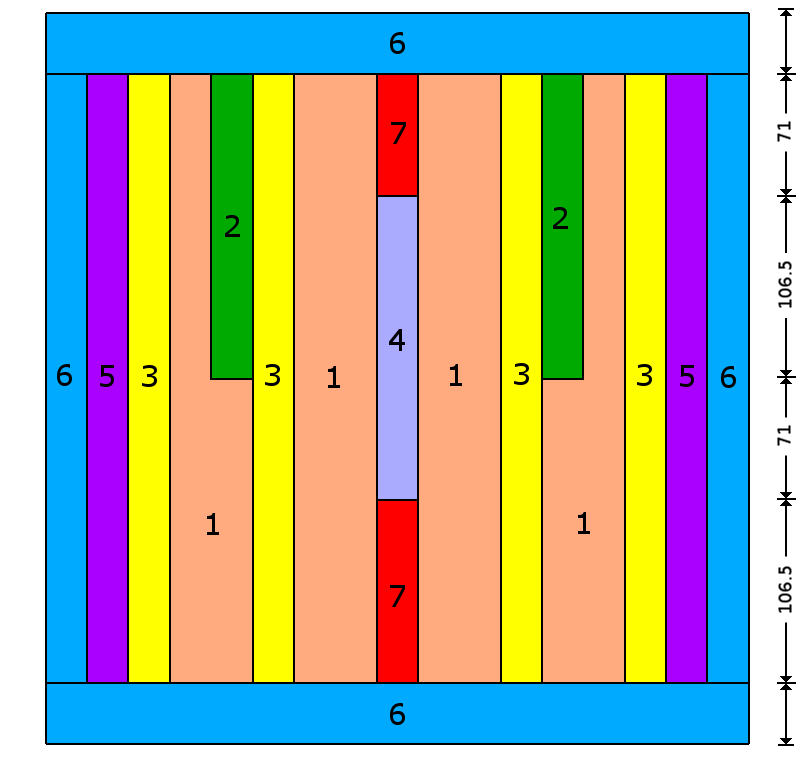
\includegraphics[width=1\linewidth] {2.png}}\\
\end{minipage}
\hfill
\caption{Radial and axial geometry of the model.}
\label{fig:1}
  \end{center}
\end{figure}


\begin{table}[h]
\caption{Diffusion neutronics constants.}
\label{t-1}
\begin{center}
\begin{tabular}{ccrrrrr}
\rowcolor{col1}
Material & Group & \multicolumn{1}{c}{$D$} & \multicolumn{1}{c}{$\Sigma_r$} & \multicolumn{1}{c}{$\Sigma_{1\to 2}$} & \multicolumn{1}{c}{$\Sigma_f$}& \multicolumn{1}{c}{$\nu\Sigma_f$}\\
\rowcolor{col3}
1 & 1 & 1.37548 & ~2.4135e-2 & ~1.5946e-2 & ~6.0130e-7 & ~4.7663e-3 \\
\rowcolor{col2}
  & 2 & 0.38333 & 6.6002e-2 &           & 1.1231e-5 & 8.3980e-2 \\
\rowcolor{col3}
2 & 1 & 1.40950 & 2.4769e-2 & 1.4346e-2 & 5.9305e-7 & 4.7020e-3 \\
\rowcolor{col2}
  & 2 & 0.38756 & 7.4988e-2 &           & 1.1253e-5 & 8.4128e-2 \\
\rowcolor{col3}
3 & 1 & 1.37067 & 2.3800e-2 & 1.5172e-2 & 7.4429e-7 & 5.8437e-3 \\
\rowcolor{col2}
  & 2 & 0.38028 & 8.0442e-2 &           & 1.5336e-5 & 1.1468e-1 \\
\rowcolor{col3}
4 & 1 & 1.39447 & 2.4069e-2 & 1.3903e-2 & 7.8731e-7 & 6.1632e-3 \\
\rowcolor{col2}
  & 2 & 0.38549 & 9.4773e-2 &           & 1.6848e-5 & 1.2598e-1 \\
\rowcolor{col3}
5 & 1 & 1.36938 & 2.3697e-2 & 1.4855e-2 & 8.1014e-7 & 6.3396e-3 \\
\rowcolor{col2}
  & 2 & 0.37877 & 8.7681e-2 &           & 1.7381e-5 & 1.2998e-1 \\
\rowcolor{col3}
6 & 1 & 1.00000 & 4.0644e-2 & 2.4875e-2 & 0.0000e-0 & 0.0000e-0 \\
\rowcolor{col2}
  & 2 & 0.33333 & 5.2785e-2 &           & 0.0000e-0 & 0.0000e-0 \\
\rowcolor{col3}
7 & 1 & 1.36966 & 2.3721e-2 & 1.4927e-2 & 7.9536e-7 & 6.2284e-3 \\
\rowcolor{col2}
  & 2 & 0.37911 & 8.5850e-2 &           & 1.6866e-5 & 1.2612e-1 \\

\end{tabular}
\end{center}
\end{table}

\section{Computional results}
In the framework of a two-group model, the spectral problem (\ref{6}) can be written as:
\begin{equation}\label{7}
\begin{split}
 - \nabla \cdot D_1 \nabla \varphi_1 & + \Sigma_{r1} \varphi_1  
 = \lambda^{(k)} (\nu \Sigma_{f1} \varphi_1 + \nu \Sigma_{f2} \varphi_2), \\
 - \nabla \cdot D_2 \nabla \varphi_2 & + \Sigma_{r2} \varphi_2 - \Sigma_{s,1\rightarrow 2} \varphi_1  
 = 0.
\end{split}
\end{equation}
The boundary conditions (\ref{2}) are used at $\gamma_g = 0.5, \ g = 1,2$.

To obtain approximate solutions we use the finite element method \cite{brenner} 
with a tetrahedron computatinal of discretization mesh. The software has been developed using the engineering and scientific calculation library FEniCS \cite{logg2012automated}. The SLEPc package \cite{slepc} has been used for the numerical solution of the spectral problems
\begin{equation}\label{8}
A\bm{x} = \lambda B \bm{x}.
\end{equation}
Used Krylov-Schur algorithm with an accuracy of $10^{-15}$. In the computations the following parameters are varied:
\begin{itemize}\itemsep1pt \parskip0pt \parsep0pt
\item the number of tetrahedrons per one assembly $\kappa$; 
\item the number of tetrahedrons in height $z$; 
\item order of finite element $p$.
\end{itemize}
The number of tetrahedrons per one assembly $\kappa$  varies from 6 to 96 and per height $z$ varies from 12 to 48. 
%Figure \ref{fig:2} shows the discretization of the assembly at $\kappa=6$ and $z=12$, $\kappa=24$ and $z=24$, $\kappa=96$ and $z=48$, respectively. 

The standard Lagrangian finite elements of degree $p=1,2,3$ are used.

%\begin{figure}[h]
%  \begin{center}
%    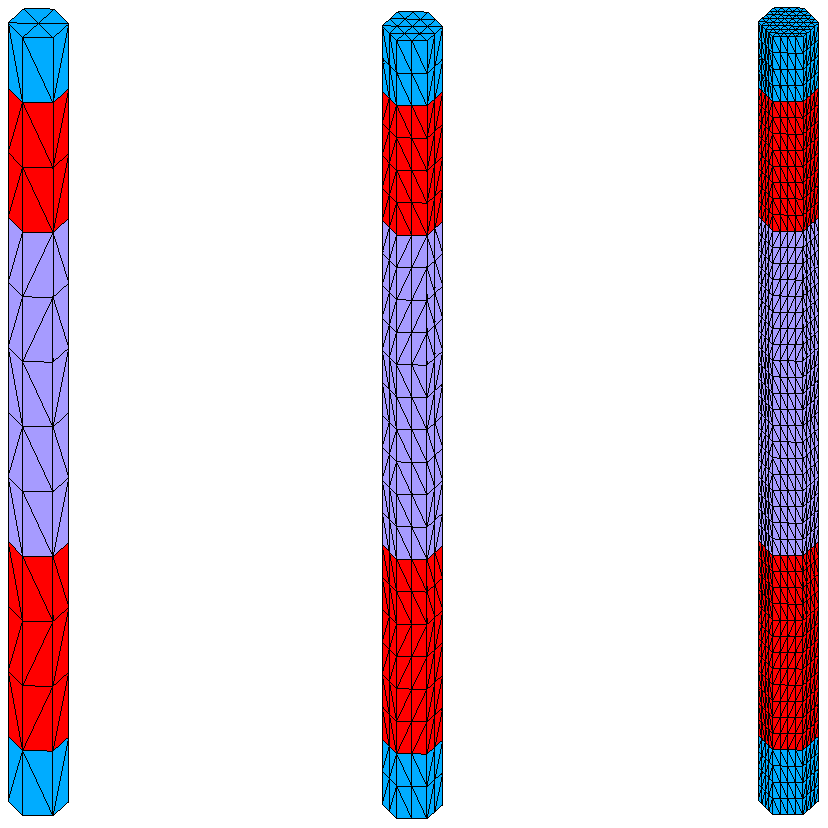
\includegraphics[width=0.35\linewidth] {3.png}
%	\caption{Different types of discretization of assembly.}
%	\label{fig:2}
%  \end{center}
%\end{figure}

The following parameters were calculated:
\begin{itemize}\itemsep1pt \parskip0pt \parsep0pt
\item the effective multiplication factor $k$;
\item the power distribution  $P$ per assembly with the normalization of the mean value of the core:
\begin{equation}\label{9}
P = a(\Sigma_{f1} \varphi_1 + \Sigma_{f2} \varphi_2),
\end{equation}
where $a$ is normalization coefficient by a given value of the integral power.
\end{itemize}

The results are compared with those, obtained using the diffusion program CRONOS \cite{cronos}. The extrapolated finite-element solution of the second-order CRONOS results is recommended as the reference solution ($k_{ref} = 1.049526$) of the Schulz benchmark. 

%CRONOS is a reactor code of CEA which uses finite elements and nodal methods for homogenized diffusion and transport calculations.
%The deviations between the CRONOS finest and extrapolated 3D solution, which characterize the accuracy of the recommended solution are given in Table 3.

Let's consider the following variations in the calculated parameters:
\begin{itemize}\itemsep1pt \parskip0pt \parsep0pt
\item for the effective multiplication factor, absolute deviation from the reference value $k_{ref}$: $\Delta k = |k - k_{ref}|$, expressed in \textit{pcm} (percent-milli, i.e. $10^{-5}$);
\item for power distribution per assembly $P_i$ calculated relative deviation $\varepsilon_i$ (expressed in \%):
\[
\varepsilon_i = \frac{P_i - P_i^{ref}}{P_i^{ref}},
\]
where $P_i^{ref}$ --- «reference» value of power per assembly $i$ ($i = 1,...,N_e$).
\item by deviations $\varepsilon_i$ calculated integral deviation:
%\begin{itemize}\itemsep1pt \parskip0pt \parsep0pt
%\item the root mean deviation RMS:
\[
\begin{split}
\mathrm{RMS} = \sqrt{\frac{1}{N_e}\sum_{i=1}^{N_e} \varepsilon_i^2}, \quad
%\]
%\item the mean absolute deviation AVR:
%\[
\mathrm{AVR} = \frac{1}{N_e}\sum_{i=1}^{N_e} \left\vert \varepsilon_i\right\vert, \quad
%\]
%\item the maximum modulus deviation MAX:
%\[
\mathrm{MAX} = \underset{i}{\max}\left\vert\varepsilon_i\right\vert.
\end{split}
\]
%\end{itemize}
\end{itemize}

Results of the solution of $\lambda$-spectral problem (\ref{6}) for the main eigenvalue $k_1 $ using different grids and finite elements are given in Table. \ref{t-2}. Here $N$ is  the size of the matrices $A,B$ (\ref{8}). These data demonstrate the convergence of the computed eigenvalues with thickening of the grid $\kappa$, $z$ and with increasing the degree $p$. Comparison of the reference solutions with the result of the solution at the parameters $p=2, \kappa=6, z=24$ (in Table \ref{t-2} highlighted in green) is shown in Figure \ref{fig:3}.


Table \ref{t-3} shows the results obtained for the next three eigenvalues for different meshes.
Vertical and horizontal cuts of power distribution for the first four eigenvalues are shown in Figure \ref{fig:4}.

\begin{table}[htp]
\caption{$k_1$ results for the Schulz benchmark.}
\label{t-2}
\begin{center}
\begin{tabular}{rrrrrrrrr}
\rowcolor{col1}
$p$ & $\kappa$ & $z$ &\multicolumn{1}{c}{$k_1$} & \multicolumn{1}{c}{$\Delta k$} & \multicolumn{1}{c}{MAX} & \multicolumn{1}{c}{AVR}& \multicolumn{1}{c}{RMS}& N \\
\rowcolor{col3}
~1& ~~6& ~12& ~1.0476057& ~192.03& ~7.9382& ~2.5145& ~2.7918& 18,278 \\
\rowcolor{col2}
1& 6& 24& 1.0484070& 111.90& 7.6614& 2.3465& 2.5983& 35,150 \\
\rowcolor{col1}
1& 6& 48& 1.0486511& 87.49& 7.6793& 2.3643& 2.6092& 68,894 \\
\rowcolor{col3}
1& 24& 12& 1.0482940& 123.20& 2.2234& 0.5665& 0.7041& 70,382 \\
\rowcolor{col3}
1& 24& 24& 1.0487937& 73.23& 1.9377& 0.4050& 0.4774& 135,350 \\
\rowcolor{col1}
1& 24& 48& 1.0493645& 16.15& 1.9823& 0.3980& 0.4612& 265,286\\
\rowcolor{col3}
1& 96& 12& 1.0483122& 121.38& 1.2015& 0.3780& 0.4857& 276,146\\
\rowcolor{col2}
1& 96& 24& 1.0490651& 46.09& 0.2647& 0.1129& 0.1389& 531,050\\
\rowcolor{col1}
1& 96& 48& 1.0493997& 12.63& 0.4554& 0.1019& 0.1243& 1,040,858\\
\rowcolor{col3}
2& 6& 12& 1.0496463& -12.03& 0.9739& 0.4801& 0.5581& 135,350\\
\rowcolor{green}
2& 6& 24& 1.0497290& -20.30& 0.9576& 0.4504& 0.5314& 265,286\\
\rowcolor{col1}
2& 6& 48& 1.0497379& -21.19& 0.9576& 0.4501& 0.5307& 525,158\\
\rowcolor{col3}
2& 24& 12& 1.0494978& 2.82& 0.3246& 0.1577& 0.1861& 531,050\\
\rowcolor{col2}
2& 24& 24& 1.0495665& -4.05& 0.2597& 0.1176& 0.1414& 1,040,858\\
\rowcolor{col1}
2& 24& 48& 1.0495858& -5.98& 0.2435& 0.1117& 0.1335& 2,060,474\\
\rowcolor{col3}
2& 96& 12& 1.0494551& 7.09& 0.1786& 0.0662& 0.0771& 2,103,650\\
\rowcolor{col2}
2& 96& 24& 1.0495265& -0.05& 0.0844& 0.0309& 0.0377& 4,123,154\\
\rowcolor{col1}
2& 96& 48& 1.0495471& -2.11& 0.0573& 0.0256& 0.0298& 8,162,162\\
\rowcolor{col3}
3& 6& 12& 1.0495750& -4.90& 0.2149& 0.0956& 0.1153& 444,962 \\
\rowcolor{col2}
3& 6& 24& 1.0495782& -5.22& 0.2110& 0.0931& 0.1125& 877,898  \\
\rowcolor{col1}
3& 6& 48& 1.0495771& -5.11& 0.2005& 0.0900& 0.1082& 1,743,770\\
\rowcolor{col3}
3& 24& 12& 1.0495406& -1.46& 0.0430& 0.0177& 0.0216& 1,756,982\\
\rowcolor{col2}
3& 24& 24& 1.0495382& -1.22& 0.0317& 0.0123& 0.0146& 3,466,478\\
\rowcolor{col1}
3& 24& 48& 1.0495381& -1.21& 0.0286& 0.0102& 0.0126& 6,885,470\\
\rowcolor{col3}
3& 96& 12& 1.0495357& -0.97& 0.0317& 0.0106& 0.0137& 6,982,418\\
\rowcolor{col2}
3& 96& 24& 1.0495338& -0.78& 0.0211& 0.0092& 0.0110& 13,776,122\\
\rowcolor{col1}
3& 96& 48& 1.0495336& -0.76& 0.0162& 0.0080& 0.0100& ~27,363,530\\
\end{tabular}
\end{center}
\end{table}

\begin{figure}[htp]
  \begin{center}
    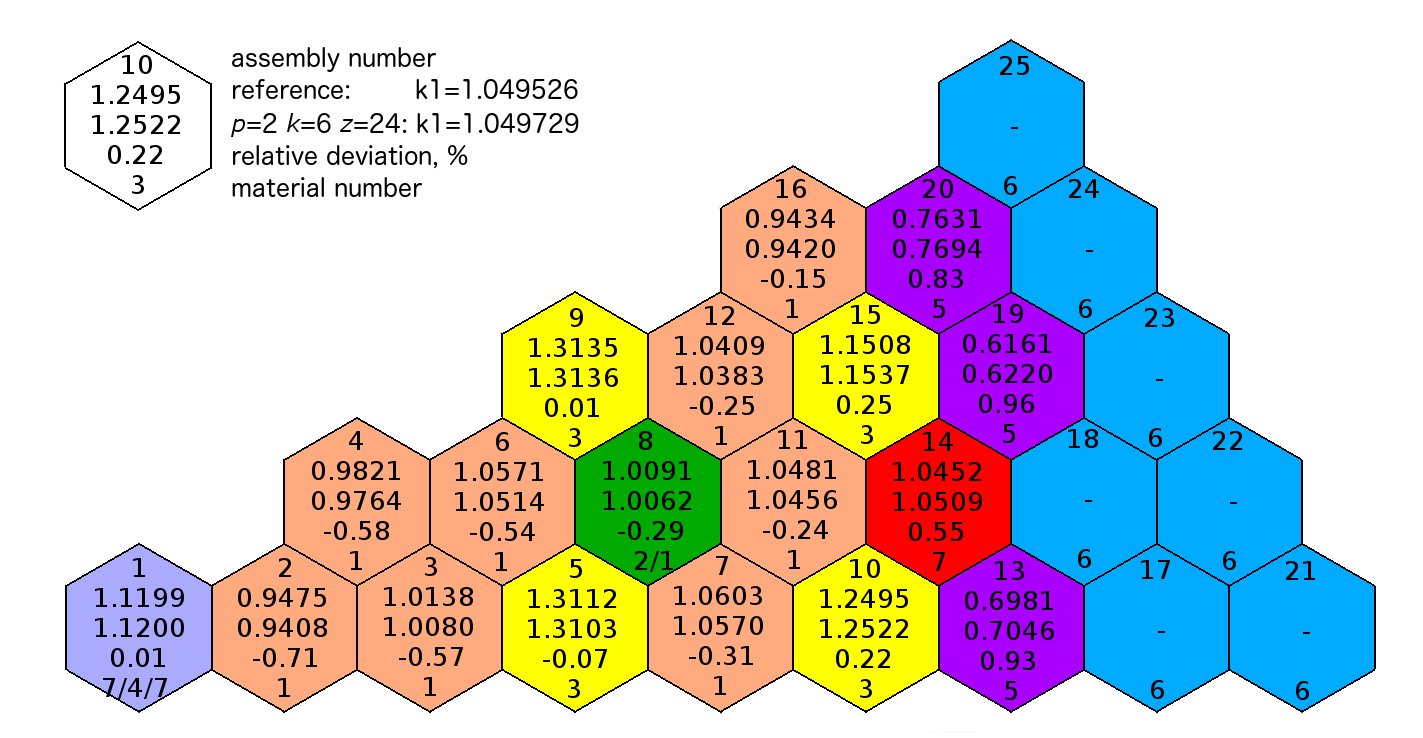
\includegraphics[width=1\linewidth] {power.png}
	\caption{Power distribution at $p=2, \kappa=6, z=24$.}
	\label{fig:3}
  \end{center}
\end{figure}

\begin{table}[htp]
\caption{The eigenvalues $k_2$, $k_3$ и $k_4$.}
\label{t-3}
\begin{center}
\begin{tabular}{rrrrrrr}
\rowcolor{col1}
$p$ & $\kappa$ & $z$ &\multicolumn{1}{c}{$k_2$} & \multicolumn{1}{c}{$k_3$} & \multicolumn{1}{c}{$k_4$} \\
\rowcolor{col3}
~1& ~~6& ~12& ~1.0367578& ~1.0367505& ~1.0265919 \\
\rowcolor{col2}
1& 6& 24& 1.0378381&	1.0378355&	1.0286801 \\
\rowcolor{col1}
1& 6& 48& 1.0381457&	1.0381434&	1.0292950\\
\rowcolor{col3}
1& 24& 12& 1.0378816&	1.0378762&	1.0277542\\
\rowcolor{col3}
1& 24& 24& 1.0389665&	1.0389631&	1.0299569\\
\rowcolor{col1}
1& 24& 48& 1.0392872&	1.0392857&	1.0306072\\
\rowcolor{col3}
1& 96& 12& 1.0378388&	1.0378365&	1.0276575\\
\rowcolor{col2}
1& 96& 24& 1.0390329&	1.0390303&	1.0300412\\
\rowcolor{col1}
1& 96& 48& 1.0393812&	1.0393798&	1.0307428\\
\rowcolor{col3}
\end{tabular}
\end{center}
\end{table}

\begin{figure}[htp]
  \begin{center}
\begin{minipage}{0.2\linewidth}
\center{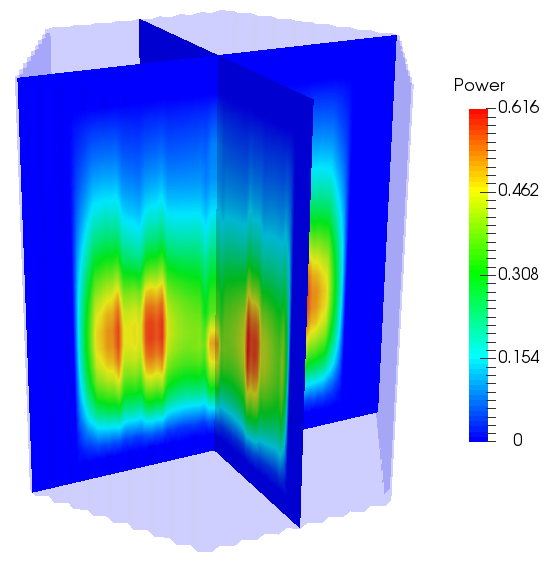
\includegraphics[width=1\linewidth]{u1v.png}}\\
vertical for $k_1$
\end{minipage}
\hfill
\begin{minipage}{0.2\linewidth}
\center{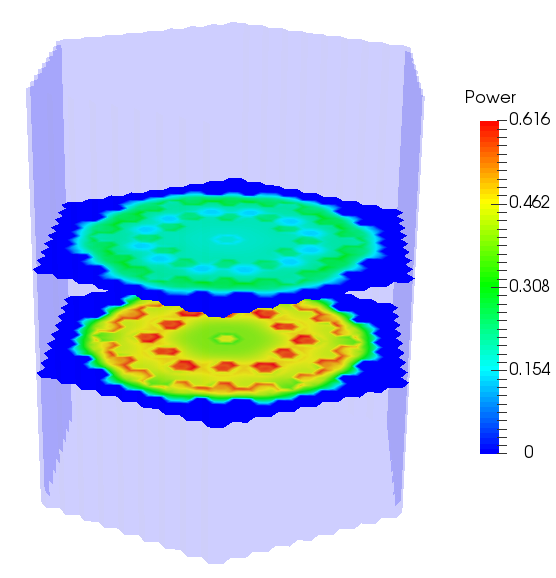
\includegraphics[width=1\linewidth]{u1h.png}}\\
horizontal for $k_1$
\end{minipage}
\hfill
\begin{minipage}{0.2\linewidth}
\center{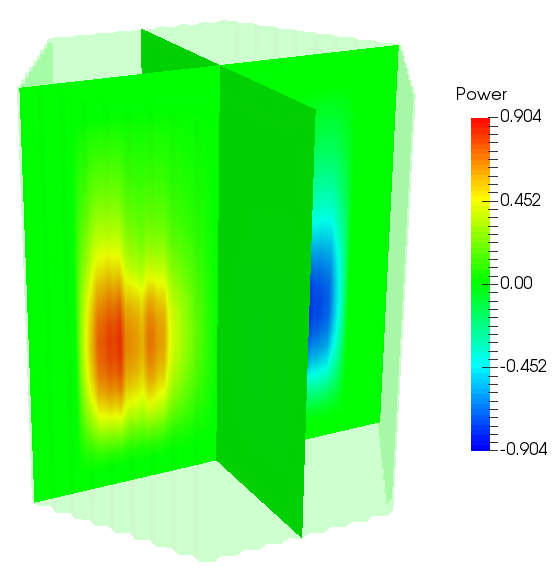
\includegraphics[width=1\linewidth]{u2v.png}}\\
vertical for $k_2$
\end{minipage}
\hfill
\begin{minipage}{0.2\linewidth}
\center{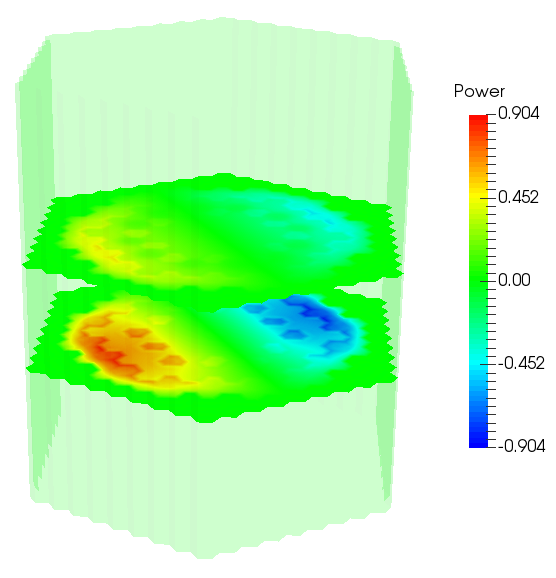
\includegraphics[width=1\linewidth]{u2h.png}}\\
horizontal for $k_2$
\end{minipage}
\vfill
\begin{minipage}{0.2\linewidth}
\center{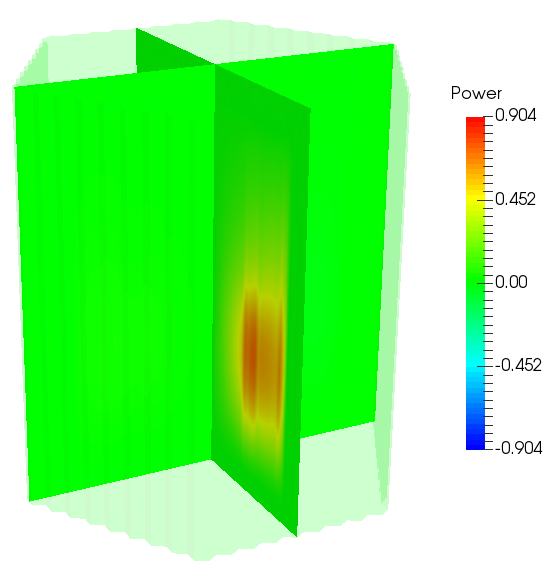
\includegraphics[width=1\linewidth]{u3v.png}}\\
vertical for $k_3$
\end{minipage}
\hfill
\begin{minipage}{0.2\linewidth}
\center{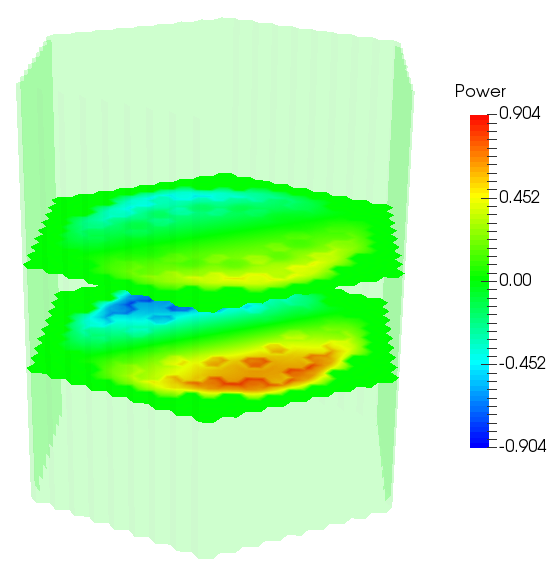
\includegraphics[width=1\linewidth]{u3h.png}}\\
horizontal for $k_3$
\end{minipage}
\hfill
\begin{minipage}{0.2\linewidth}
\center{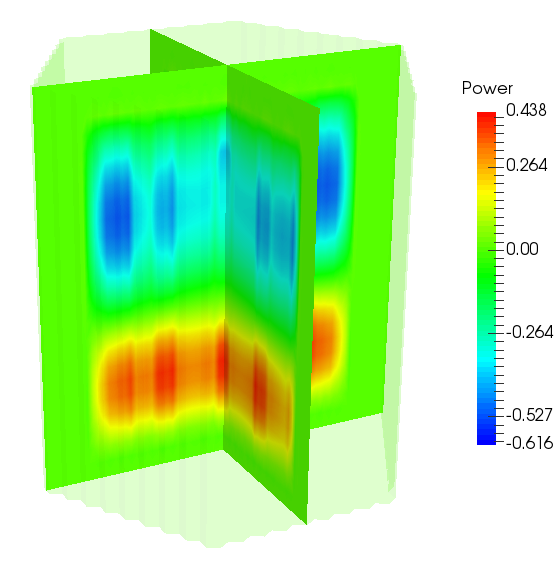
\includegraphics[width=1\linewidth]{u4v.png}}\\
vertical for $k_4$
\end{minipage}
\hfill
\begin{minipage}{0.2\linewidth}
\center{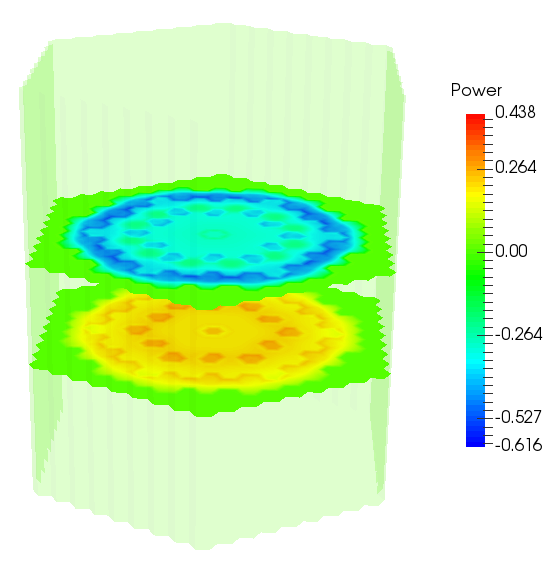
\includegraphics[width=1\linewidth]{u4h.png}}\\
horizontal for $k_4$
\end{minipage}

\caption{Sections.}
\label{fig:4}
  \end{center}
\end{figure}

\section{Summary}
In this paper we have performed computational analysis of the 3D neutron diffusion benchmark of a VVER-1000 core. The software has been developed using the engineering and scientic library FEniCS and the matrix spectral problem is solved using the SLEPc package. The number of tetrahedrons per assembly $\kappa$ varies from 6 to 96; the number of tetrahedrons in height $z$ varies from 12 to 48. The finite elements of degree $p$ = 1, 2, 3 are used. The results are compared with the extrapolated finite-element solution of the second-order CRONOS results recommended as the reference solution. An excellent agreement of the results was obtained for the maximum values of the parameters ($\kappa$=96, $z$=48 and $p$=3). There are deviations in the results at the rounding error level. In the practice of engineering calculations it is sufficient to use the following parameters: $\kappa$=6, $z$=24 and $p$=2. The results can be useful for the diffusion codes intercomparison.

\section{Acknowledgements}
The research was supported by the Government of the Russian Federation (project 14.Y26.31.0013).

\begin{thebibliography}{12}
\bibitem{duderstadt1976nuclear}
Duderstadt, J.J., Hamilton, L.J.: Nuclear Reactor Analysis. Wiley (1976)

\bibitem{stacey2007}
Stacey, W.M.: Nuclear Reactor Physics. Wiley (2007)

\bibitem{hetrick1971dynamics}
Hetrick, D.L.: Dynamics of Nuclear Reactors. University of Chicago Press (1971)

\bibitem{marchuk1986numerical}
Marchuk, G.I., Lebedev, V.I.: Numerical Methods in the Theory of Neutron Transport. Harwood Academic Pub  (1986)

\bibitem{lewis1993computational}
Lewis, E.E., Miller, W.F.: Computational Methods of Neutron Transport. American Nuclear Society (1993)

\bibitem{publicAnnnals2017}
Avvakumov, A.V., Vabishchevich, P.N., Vasilev, A.O., Strizhov, V.F.: Spectral properties of dynamic processes in a nuclear reactor. Annals of Nuclear Energy, vol. 99, pp. 68--79 (2017)

\bibitem{schulz1996}
Schulz, G.: Solution of a 3D VVER-1000 benchmark. In Proc. of 6-th Symposium of AER, Kikkonummi, Finland (1996)

\bibitem{brenner}
Brenner, S.C., Scott, R.: The Mathematical Theory of Finite Element Methods. Springer (2008)

\bibitem{logg2012automated}
Logg, A., Mardal, K.A., Wells, G.: Automated solution of differential equations by the finite element method: The FEniCS book. Springer Science \& Business Media, vol. 84 (2012)

\bibitem{slepc}
Campos, C., Roman, J.E., Romero, E., Tomas, A.: SLEPc Users Manual, \url{http://slepc.upv.es/documentation/manual.htm} (2013)

\bibitem{cronos}
Kolev, N.P., Lenain, R., Fedon-Magnaud, C.: Solutions of the AER 3D Benchmark for VVER-1000 by CRONOS”. Proc. 7-th Symposium of AER on VVER Reactor Physics and Safety, Hoernitz, Germany (1997)
  
\end{thebibliography}


\end{document}
